% ch05-ml.tex -- Trees and ensembles
\chapter{Trees and ensembles}\label{ch:trees}

A decision tree\index{decision tree} is a program you could read aloud:
``if \texttt{color\_intensity} $\le 3.800$, go left; else go right'' ---
a chain of axis-aligned yes/no questions ending in a majority vote. It is
the first model in the book whose learned structure is itself
interpretable, and it is also the first that overfits almost on purpose:
grown deep enough, a tree reproduces its training set perfectly. The
second half of the chapter is the fix, and it is one of the most
profitable ideas in the field: \emph{train many flawed trees and average
them}. Bagging, random forests, and gradient boosting are three ways to
spend the same insight --- reduce variance by voting --- and together they
power most of the tabular machine learning actually deployed. Below we
grow a tree by hand, measure a single tree's variance over 20 bootstraps,
and watch boosting fit residuals stage by stage.

\section{Trees as axis-aligned partitions}\label{sec:treedef}

A tree carves feature space into rectangles\index{partition}: each
internal node tests one feature against one threshold, each leaf predicts
the majority class (or mean target) of its cell. The picture to hold is
the correspondence: every tree is a staircase partition, every staircase
partition is some tree.

\begin{figure}[ht]\centering
\begin{tikzpicture}[font=\small]
  % left: the tree
  \begin{scope}[shift={(0,0)}]
    \node[draw] (r) at (0,0) {$x_1 \le t_1$};
    \node[draw, below left=0.7cm and 0.9cm of r] (a) {$x_2 \le t_2$};
    \node[draw, below right=0.7cm and 0.9cm of r] (b) {$x_2 \le t_3$};
    \node[draw, below left=0.7cm and 0.45cm of a, minimum width=0.9cm] (l1) {$A$};
    \node[draw, below right=0.7cm and 0.45cm of a, minimum width=0.9cm] (l2) {$B$};
    \node[draw, below left=0.7cm and 0.45cm of b, minimum width=0.9cm] (l3) {$C$};
    \node[draw, below right=0.7cm and 0.45cm of b, minimum width=0.9cm] (l4) {$D$};
    \draw[->] (r) -- (a) node[midway, left, font=\scriptsize]{yes};
    \draw[->] (r) -- (b) node[midway, right, font=\scriptsize]{no};
    \draw[->] (a) -- (l1); \draw[->] (a) -- (l2);
    \draw[->] (b) -- (l3); \draw[->] (b) -- (l4);
  \end{scope}
  % right: the partition
  \begin{scope}[shift={(6.0,-0.8)}]
    \draw (0,0) rectangle (3.4,3.4);
    \draw (1.4,0) -- (1.4,3.4) node[below, font=\scriptsize]{$t_1$};
    \draw (0,1.9) -- (1.4,1.9) node[left, font=\scriptsize]{$t_2$};
    \draw (1.4,1.1) -- (3.4,1.1) node[right, font=\scriptsize]{$t_3$};
    \node at (0.7,2.6) {$A$}; \node at (0.7,0.95) {$B$};
    \node at (2.4,2.25) {$C$}; \node at (2.4,0.55) {$D$};
  \end{scope}
\end{tikzpicture}
\caption{Tree $\leftrightarrow$ partition. Each split is one axis-aligned
cut; every path root-to-leaf is one rectangle of feature space. Depth-2
here; a real tree recurses the same two moves.}\label{fig:treepartition}
\end{figure}

\section{Choosing a split: Gini and information gain}\label{sec:splitcrit}

Greedy induction asks, at each node, one question: \emph{which
(feature, threshold) pair makes the children purest?} Purity is measured
by the Gini impurity\index{Gini impurity}
\[
G(\text{node}) = 1 - \sum_c p_c^2
\]
(the probability a random label disagrees with a random draw), or
equivalently-ranked entropy. A split's score is the weighted-impurity
drop --- \emph{information gain}\index{information gain}:
\[
\Delta = G(\text{parent}) -
\frac{n_L}{n}G(\text{left}) - \frac{n_R}{n}G(\text{right}).
\]

\lstinputlisting[language=Python,caption={\texttt{code/ch05/tree\_scratch.py}: recursive growth --- best threshold over every feature, Gini gain, depth cap, leaf majority.},label={lst:tree}]{code/ch05/tree_scratch.py}

\lstinputlisting[numbers=none]{code/ch05/tree_scratch.out.txt}

\begin{example}[WE 5.1 --- The first split, computed by hand]\label{ex:ig}
Strategy: verify the tree's root decision arithmetic yourself.\par
\begin{solution}
On \texttt{wine} train ($n{=}133$: 44/53/36 per class), root Gini is
$1 - (0.331^2 + 0.398^2 + 0.271^2) = 0.6585$. The winning split
\texttt{color\_intensity} $\le 3.8$ produces a left child of
$n{=}49$ (3/46/0, $G{=}0.115$) and a right child of $n{=}84$
(41/7/36, $G{=}0.571$); weighted children $= 0.403$ and gain
$0.6585 - 0.403 = 0.2554$ --- exactly what the tree prints. Left is nearly
pure already; the tree has found, in one cut, the feature that separates
the middle class.
\end{solution}
\end{example}

\begin{figure}[ht]\centering
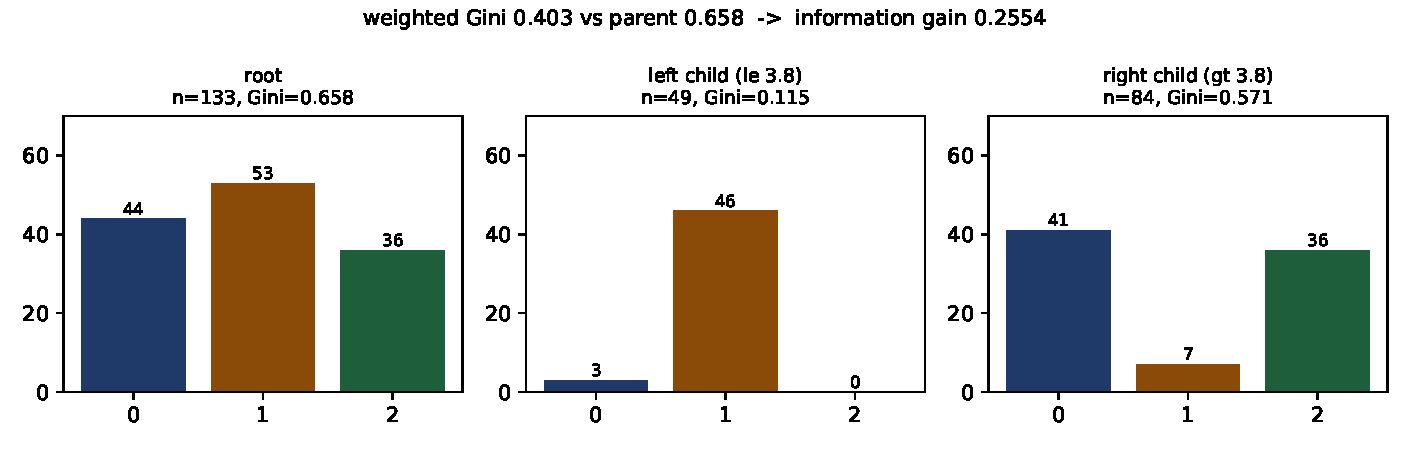
\includegraphics[width=\linewidth]{figures/ch05/ig_panel.pdf}
\caption{WE 5.1 as a picture (\texttt{figures/fig\_ch05\_ig\_panel.py}):
parent and two children, class counts and Gini each --- the weighted drop
is the split's score.}\label{fig:igpanel}
\end{figure}

\section{Growing, depth, and the overfit cliff}\label{sec:depth}

The recursion stops on purity or a depth cap; prune it\index{pruning} and
the tree trades memorisation for shape. Listing~\ref{lst:forest}'s depth
sweep is the bias--variance story again, written in branches: depth-2
underfits (test $0.307$), depth-6 is sane ($0.751$), depth-10 hits
$0.856$ test while train accuracy is already $0.976$ --- and full depth
memorises train at $1.000$ while test \emph{falls} to $0.849$.

\lstinputlisting[language=Python,caption={\texttt{code/ch05/forest\_lib.py}: one tree's variance over 20 bootstrap refits, the depth sweep, then the 300-tree forest.},label={lst:forest}]{code/ch05/forest_lib.py}

\lstinputlisting[numbers=none]{code/ch05/forest_lib.out.txt}

\section{Bagging: vote across bootstrap worlds}\label{sec:bagging}

\index{bagging}A single deep tree is all variance: retrain it on a
bootstrap resample\index{bootstrap} and the answer moves --- mean
$0.824$, sd $0.018$ over 20 refits in the listing. But averaging the 20
answers cancels the disagreement: variance of a mean of $B$ decorrelated
learners falls like $1/B$. That is the whole trick of bagging (and the
random forest\index{random forest}, which adds feature subsampling per
split to decorrelate further). The listing's verdict: lone tree $0.849$,
300-tree forest $0.982$ --- $13$ points of test accuracy, free, no tuning.

\begin{figure}[ht]\centering
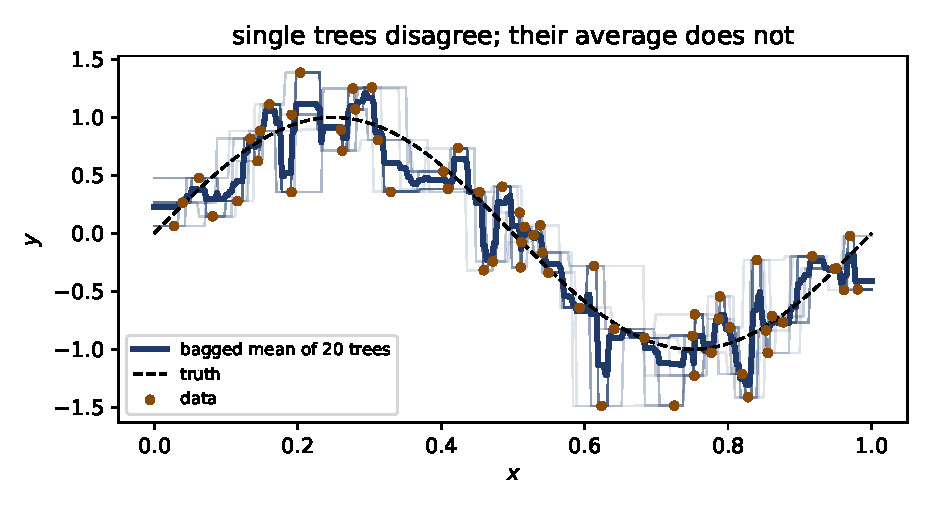
\includegraphics[width=0.7\linewidth]{figures/ch05/bagging_overlay.pdf}
\caption{20 trees fit bootstrap-resampled data
(\texttt{figures/fig\_ch05\_bagging\_overlay.py}): each staircase is
different (variance), their mean tracks the truth (cancelled). Bagging is
exactly this picture at scale.}\label{fig:bagging}
\end{figure}

\section{Gradient boosting: residuals as targets}\label{sec:boosting}

\index{gradient boosting}Boosting asks a different question of the same
lego: instead of independent trees, build a chain where each new tree is
fit on the \emph{residuals} of the ensemble so far --- a gradient step in
function space. Listing~\ref{lst:boost} shows the loop raw: predict the
mean, then at each stage fit a small tree to what the ensemble still gets
wrong, scaled by a learning rate.

\lstinputlisting[language=Python,caption={\texttt{code/ch05/boost\_compare.py}: boosting by hand on \texttt{california} (RMSE stage by stage), then scratch-vs-library on the same split.},label={lst:boost}]{code/ch05/boost_compare.py}

\lstinputlisting[numbers=none]{code/ch05/boost_compare.out.txt}

\begin{example}[WE 5.2 --- Residual shrinkage, stage by stage]\label{ex:boost}
Strategy: read the RMSE trace as function-space gradient descent.\par
\begin{solution}
Stage 0 predicts the mean (test RMSE $1.161$). Each depth-3 tree carves
off a chunk of the remaining error at lr $0.3$: $0.994$, $0.890$,
$0.777$, $0.655$, $0.582$ by stage 16 --- still shrinking, never fitting
train. And the library comparison on the same split: single tree
$R^2{=}0.604$, random forest $0.801$, \texttt{HistGradientBoosting}
$0.828$. Boosting and bagging both beat one tree --- boosting by
\emph{correcting} errors serially, bagging by \emph{averaging} them in
parallel.
\end{solution}
\end{example}

\begin{figure}[ht]\centering
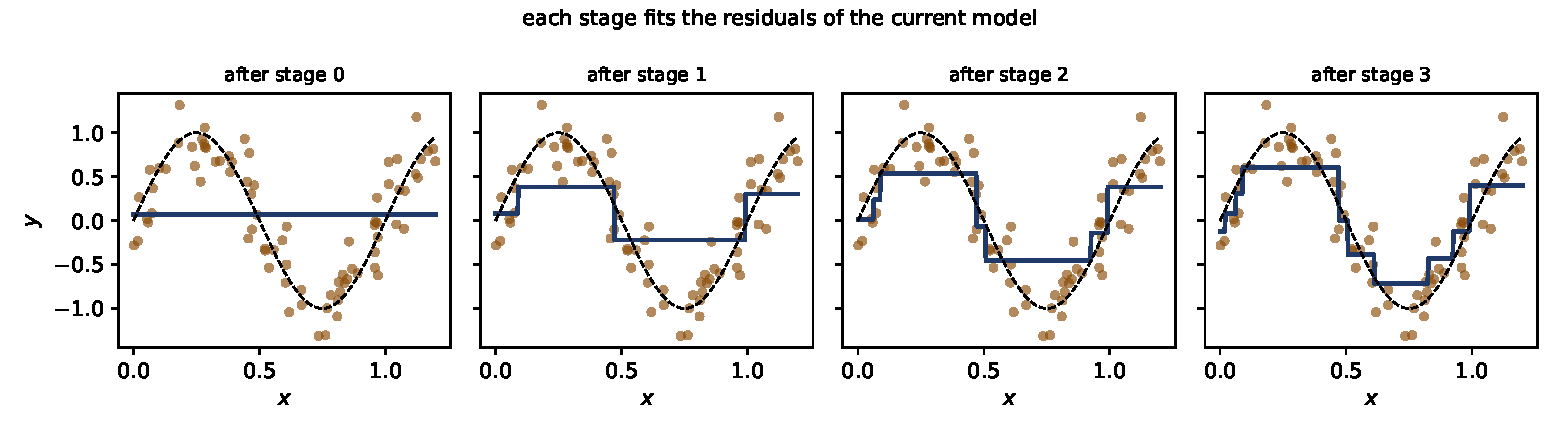
\includegraphics[width=\linewidth]{figures/ch05/boost_seq.pdf}
\caption{Boosting stage-by-stage on 1-D synthetic data
(\texttt{figures/fig\_ch05\_boost\_seq.py}): each panel adds one
residual-fitting tree; the ensemble's staircase sharpens where the last
stage failed.}\label{fig:boostseq}
\end{figure}

\section{Feature importance --- and when it lies}\label{sec:importance}

\index{feature importance}Two importance scores in common use tell
different stories. \emph{MDI} (mean decrease in impurity) credits a
feature with the impurity it removed at splits --- cheap, biased toward
high-cardinality features, computed on training data. \emph{Permutation
importance} shuffles one column on test and measures the accuracy drop
--- honest, expensive, and the one to trust. The trap: correlated
features \emph{split the vote} --- a redundant duplicate of the top
feature steals half its credit under either score.

\begin{figure}[ht]\centering
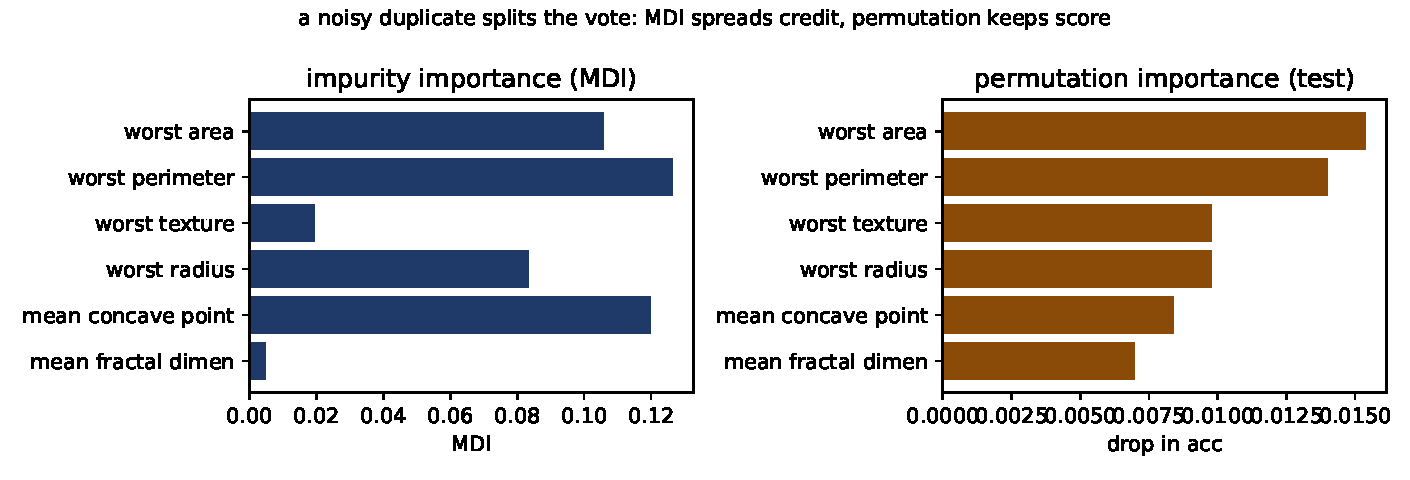
\includegraphics[width=\linewidth]{figures/ch05/importance_illusion.pdf}
\caption{The importance illusion, planted and measured
(\texttt{figures/fig\_ch05\_importance\_illusion.py}): a noisy duplicate
of \texttt{worst concave points} joins the data and both metrics split
credit between the pair --- the ranking survives, the magnitudes lie.
Report the score, name the method, and beware redundancy.}\label{fig:importance}
\end{figure}

\begin{example}[WE 5.3 --- The dilution, measured]\label{ex:dilution}
Strategy: plant the duplicate, fit, and ask the forest who did the work.
\par
\begin{solution}
Figure~\ref{fig:importance} shows the ranking intact --- \texttt{worst
concave points} still tops --- but its credit is now shared with the
dup, and every other feature's \emph{relative} importance is inflated
by comparison. MDI and permutation agree on the order yet disagree on
the margin. Interpretation lesson: importance is a statement about the
\emph{model's use} of a feature, not the feature's role in the world
--- a correlated column can be causally crucial and rank low.
\end{solution}
\end{example}

\begin{wins}
What you can now do: grow a tree by hand with Gini gain; read depth as a
bias--variance dial; explain bagging/forest/boosting as three ways to
spend the averaging idea; tell MDI from permutation importance and spot
the correlation dilution.
\end{wins}

\section{Common mistakes}

\begin{description}
\item[Growing to full depth ``because it fits''] $1.000$ train accuracy
  on a tree is the warning, not the win --- cap depth, min-samples-leaf,
  or prune by cost-complexity.
\item[Trusting feature importance as causal] Importance scores the
  model's habits, not the feature's role --- correlated or leaky columns
  distort it in either direction.
\item[Bagging when boosting fits, boosting when bagging fits] Bagging
  cures variance; boosting cures bias-ish error. Diagnose the gap on the
  learning curve before choosing the ensemble.
\item[Forgetting the random seed in trees] One
  \texttt{DecisionTree} \texttt{Classifier} is a lottery draw across
  refits --- never judge a split from one seed.
\item[Evaluating OOB on test too] OOB\index{out-of-bag} is a free
  validation set inside the forest; do not double-dip --- it is not a
  substitute for the sealed test set when tuning.
\item[Deep boosting trees] Boosting wants shallow (depth 1--4): the
  ensemble is the depth. A deep base learner overfits before the chain
  can correct it.
\item[Ignoring scale invariance] Trees do not need standardised
  features --- thresholds are scale-free. Save the preprocessing effort
  for the models that need it.
\item[Reading MDI on high-cardinality data] A near-unique ID column wins
  every split and tops MDI --- the known bias; use permutation or drop
  the column.
\item[Boosting with a huge learning rate] lr is a shrinkage dial; at
  1.0 the chain oscillates, at 0.05 it needs 10$\times$ the trees ---
  tune it with the tree count together.
\end{description}

\section{Summary table}

\begin{tabularx}{\linewidth}{@{}l l X@{}}
\toprule
\textbf{Idea} & \textbf{Mechanism} & \textbf{When it wins}\\
\midrule
Single tree & recursive Gini/entropy splits & interpretable small problems\\
Bagging & bootstrap $+$ average & kill variance of one unstable learner\\
Random forest & bagging $+$ feature subsample & the default tabular answer\\
Gradient boost & sequential residual fitting & top accuracy on clean tabular\\
HistGB/XGBoost & histogram-speed boosting & scale + missing values\\
Depth/min-leaf & capacity dials & prune or cap, always\\
Importance & MDI vs permutation & report which; beware redundancy\\
\bottomrule
\end{tabularx}

\section{Drill --- five concept questions}

\begin{enumerate}
\item Bagging reduces which of bias or variance --- and what makes the
  average fall like $1/B$?
\item A random forest adds one ingredient on top of bagging. Name it and
  what it decorrelates.
\item In boosting, what is each new tree's target --- and what does the
  learning rate control?
\item MDI credits a near-unique-ID column top importance. What does
  permutation importance say instead, and why?
\item Full-depth tree: train $1.000$, test $0.849$. Depth-10: train
  $0.976$, test $0.856$. Which is deployed, and what do the two numbers
  diagnose?
\end{enumerate}

\section*{Further reading}
\begin{itemize}
\item Breiman --- ``Random Forests,'' \emph{Machine Learning} 45 (2001).
  \url{https://www.stat.berkeley.edu/~breiman/randomforest2001.pdf} ---
  the original, still the best single read on why subsampling works.
\item scikit-learn --- \emph{Ensembles} user guide.
  \url{https://scikit-learn.org/stable/modules/ensemble.html} ---
  RandomForest, HistGB, and friends as used in the listings.
\item Friedman --- ``Greedy Function Approximation: A Gradient Boosting
  Machine,'' \emph{Annals of Statistics} 29 (2001).
  \url{https://projecteuclid.org/journals/annals-of-statistics/volume-29/issue-5/Greedy-function-approximation-A-gradient-boosting-machine/10.1214/aos/1013203451.full}
  --- gradient descent in function space, from the source.
\item Chen \& Guestrin --- ``XGBoost: A Scalable Tree Boosting System,''
  KDD 2016. \url{https://arxiv.org/abs/1603.02754} --- the systems
  engineering that made boosting the tabular standard.
\item scikit-learn --- \emph{Permutation importance}.
  \url{https://scikit-learn.org/stable/modules/permutation_importance.html}
  --- the honest importance score; WE~5.3's method.
\item XGBoost documentation. \url{https://xgboost.readthedocs.io/en/stable/}
  --- parameters that map one-to-one onto the chapter's concepts.
\item LightGBM documentation. \url{https://lightgbm.readthedocs.io/en/stable/}
  --- leaf-wise growth and GOSS; the other production booster.
\end{itemize}

\begin{rulebox}{Watch instead (if you'd rather see it)}
\begin{itemize}
\item \textbf{StatQuest: Decision and Classification Trees, Clearly
  Explained} (18:08). StatQuest with Josh Starmer.
  \url{https://www.youtube.com/watch?v=_L39rN6gz7Y} --- Gini walkthrough
  matching \S\ref{sec:splitcrit} and WE~5.1. Accessed 2026-10-11.
\item \textbf{StatQuest: Random Forests Part 1 --- Building, Using and
  Evaluating} (9:54). StatQuest with Josh Starmer.
  \url{https://www.youtube.com/watch?v=J4Wdy0Wc_xQ} --- bagging intuition
  matching \S\ref{sec:bagging}. Accessed 2026-10-11.
\item \textbf{StatQuest: Gradient Boost Part 1 --- Regression Main
  Ideas} (15:52). StatQuest with Josh Starmer.
  \url{https://www.youtube.com/watch?v=3CC4N4z3GJc} --- residual-fitting
  sequence matching \S\ref{sec:boosting} and WE~5.2. Accessed 2026-10-11.
\end{itemize}
\end{rulebox}

\chapternotes
\begin{enumerate}
\item CART (Breiman et al.\ 1984) is the lineage every library here
  implements; ID3/C4.5 (Quinlan) used entropy and is the historical
  sibling.
\item Random forests subsample features per split precisely to
  decorrelate the voters --- a single dominant feature would otherwise
  appear in every tree and the $1/B$ dream dies.
\item XGBoost's engineering (approximate splits, cache-aware layout,
  regularised objectives) is why it took the tabular crown; the maths is
  the same gradient boosting.
\item OOB is nearly-free validation: each tree skips $\approx 36.8\%$ of
  rows ($1/e$ of draws), so scoring each row on its non-voters estimates
  generalisation --- see sklearn's \texttt{oob\_score}.
\item MDI's high-cardinality bias is documented in sklearn's
  permutation-importance guide (Further reading); WE~5.3 reproduces the
  mechanism rather than trusting the docs.
\end{enumerate}

\section*{Exercises}

\emph{[easy]}
\begin{exercise}
Compute the Gini of a node with class counts (10, 5), then of a split
producing (8, 0) and (2, 5). What is the gain?
\end{exercise}
\begin{exercise}
Which ensemble reduces variance but not bias, and which reduces both in
effect? Name each.
\end{exercise}
\begin{exercise}
In WE~5.1, the left child's Gini is 0.115. Verify it from the counts
(3/46/0).
\end{exercise}
\begin{exercise}
What does a depth-1 tree (a \emph{stump}) correspond to in the
partition picture? Why does boosting like stumps?
\end{exercise}

\emph{[medium]}
\begin{exercise}
Extend Listing~\ref{lst:tree} to support entropy splits; grow the same
tree and diff the structure with the Gini one.
\end{exercise}
\begin{exercise}
Implement OOB scoring on the \texttt{digits} forest: score each row by
the trees that did not train on it, and compare with the sealed test
accuracy.
\end{exercise}
\begin{exercise}
Run the depth sweep of Listing~\ref{lst:forest} with
\texttt{min\_samples\_leaf=5}; how does the optimum depth shift?
\end{exercise}
\begin{exercise}
Reproduce Figure~\ref{fig:bagging} on \texttt{california} (project to
one feature or average predictions across features) and quantify the
bagged model's RMSE gain over the mean single tree.
\end{exercise}
\begin{exercise}
Plant the WE~5.3 duplicate on \texttt{digits} and measure how the top-5
permutation ranking changes vs the clean data.
\end{exercise}
\begin{exercise}
Implement column subsampling in the scratch tree (split search over
$\sqrt{d}$ random features per node) and measure the test-accuracy
effect on the same split.
\end{exercise}

\emph{[hard]}
\begin{exercise}
Prove Gini is an impurity upper bound on classification error: at a
node predicting the majority class, $G \ge \epsilon$ where
$\epsilon$ is the local error rate. When is equality achieved?
\end{exercise}
\begin{exercise}
Derive that for squared loss, the optimal leaf value at a node is the
mean of its targets --- and the next boosting step then fits residuals
exactly.
\end{exercise}
\begin{exercise}
Design the experiment that separates ``the forest is good'' from ``the
features are easy'': swap in a duplicate-only feature set and measure
which score (MDI, permutation, accuracy) moves first.
\end{exercise}
\begin{exercise}
Show the boosting step is a gradient step: write squared-loss
$-\partial L/\partial F$, show it equals the residual, and conclude why
``fit residuals'' is really ``descend in function space.''
\end{exercise}
\begin{exercise}
Build a correlation-dilution study: sweep the number of planted
duplicates of the top feature and plot its permutation importance ---
predict the curve before you run it.
\end{exercise}

\section*{Hints and answers}
\begin{description}
\item[5.1] $1 - (0.667^2 + 0.333^2) = 0.444$; children $0$ and $0.36$;
  gain $\approx 0.23$.
\item[5.2] Bagging: variance only. Boosting: bias (mainly) --- the chain
  adds capacity serially.
\item[5.3] $1 - (3/49)^2 - (46/49)^2 - 0 = 0.115$.
\item[5.4] One cut, two rectangles --- boosting's weak learners stay
  weak so the chain stays honest.
\item[5.5] Replace the impurity with
  $-\sum p\log p$; expect near-identical trees (the criteria rarely
  differ in rank order).
\item[5.6] Each training row is OOB for $\approx 36.8\%$ of trees.
\item[5.7] Larger min-leaf $\Rightarrow$ shallower optimum; the
  regularisation moves the cliff left.
\item[5.8] Bagged RMSE usually lands 5--15\% below the single-tree mean;
  report the spread too.
\item[5.9] The dup splits the top feature's credit; rankings below it
  shift up a slot.
\item[5.10] Column subsampling lowers single-tree accuracy but improves
  the forest's --- decorrelation is the point.
\item[5.11] Majority predictor error is $1 - p_{\max}$; $G \ge 1 -
  p_{\max}$ iff $p_{\max} \ge p_{\max}^2$, equality at purity or
  $p_{\max}{=}0.5$ in binary.
\item[5.12] $\partial \sum (y_i - c)^2/\partial c = 0 \Rightarrow c =
  \bar y$; residual fit then equals the next gradient step.
\item[5.13] Accuracy should hold while MDI swings --- the decoy proves
  which metric is honest.
\item[5.14] $-\partial L/\partial F = 2(y - F) \propto$ residual; the
  step direction is the pseudo-residual.
\item[5.15] Importance falls like $\approx 1/(k+1)$ in $k$ duplicates;
  test your prediction against the plot.
\end{description}
